%Основная шапка, без которой невозможно собрать документ
\documentclass[a4paper,14pt,russian]{extreport}		%хотим создать класс документа "статья" с основным шрифтом 12
\usepackage[utf8]{inputenc}			%в какой кодировке пишем
\usepackage[T2A]{fontenc}			%какой используем буквенный формат
\usepackage[russian]{babel}			%на каком языке пишем
%эти 4 строки должны быть в начале каждого документа в ТеХе, без них документ не соберется. Все что дальше - бонусы для красоты или удобства.

\usepackage[pdftex]{geometry}		%пакет для пользовательской настройки геометрии листа и текста
\geometry{	paperheight=28.5cm, 	%высота листа
			paperwidth=21cm, 		%ширина листа
			top=1.5cm, 				%отступ сверху
			bottom=1.6cm,			%отступ снизу
			left=2cm, 				%отступ слева
			right=2cm, 				%отступ справа
			headheight=0.8cm, 		%высота колонтикула
			headsep=0.9cm, 			%отступ от колонтикула
			footskip=1cm}			%отступ снизу для ссылок\номеров страниц и тд

%Так вызываются пакеты для использования в тексте определенного наполнения. Обычно достаточно вызвать пакет, если его нет в системе, происходит автоматическая скачка с серверов LaTex.
\usepackage{subfigure}
\usepackage{amsmath}                %специальные математические функции
\usepackage{amsfonts}               %специальные математические символы
\usepackage{graphicx}               %пакет для вставки рисунков
\usepackage{csquotes} 				%красивые кавычки специальной функцией
\renewcommand{\sectionmark}[1]{\markboth{#1}{}}
\newcommand{\cev}[1]{\reflectbox{\ensuremath{\vec{\reflectbox{\ensuremath{#1}}}}}}
\usepackage{graphicx} % для вставки картинок
\usepackage{amssymb,amsfonts,amsmath,amsthm} % математические дополнения от АМС
\usepackage{indentfirst} % отделять первую строку раздела абзацным отступом тоже
\usepackage[usenames,dvipsnames]{color} % названия цветов
\usepackage{makecell}
\usepackage{multirow} % улучшенное форматирование таблиц
\usepackage{ulem} % подчеркивания

\usepackage{braket}
\usepackage{fancyhdr}
\usepackage{setspace}

\usepackage[percent]{overpic}

\usepackage{biblatex} %Imports biblatex package
\addbibresource{refs.bib} %Import the bibliography file
\usepackage{bm}

% Полуторный интервал
\onehalfspacing
%Функции для определения размеров шрифта. Первая цифра текстовой шрифт, вторая - основной шрифт формул, третья - размер индексов, четвертая - размер индексов у индексов. 
\DeclareMathSizes{10}{9}{5}{5}          %for 10pt font size
\DeclareMathSizes{11}{9}{5}{5}         	%for 11pt font size
\DeclareMathSizes{12}{11}{6}{6}         %for 12pt font size

%Две функции, контролирующие переносы и разрывы строк. Обычно ставлю всегда, не изменяя значений.
\hyphenpenalty 500
\fussy

\newcommand{\HRule}{\rule{\linewidth}{0.2mm}} 	%специальная ручная команда для линии в титульнике. В документах без линии не нужна

% custom
\newtheorem{theorem}{Теорема}
\newtheorem{definition}{Опр.}
\newtheorem{lemma}{Лемма}
\usepackage{bbold}

\usepackage{physics}

\begin{document}
\begin{center}			
{\small ФЕДЕРАЛЬНОЕ ГОСУДАРСТВЕННОЕ БЮДЖЕТНОЕ ОБРАЗОВАТЕЛЬНОЕ УЧРЕЖДЕНИЕ ВЫСШЕГО ОБРАЗОВАНИЯ <<МОСКОВСКИЙ ГОСУДАРСТВЕННЫЙ УНИВЕРСИТЕТ имени М.В.ЛОМОНОСОВА>>}
\end{center}
\vspace*{-1cm}
\begin{center}
\HRule
\end{center}

\begin{center}
Физический факультет\\Кафедра квантовой статистики и теории поля\\[5cm]
\end{center}

\begin{center}
Дипломная работа\\студента Дмитриева Е.М.\\
на тему
\end{center}

\begin{center}
Асимптотическая сцепленность в квантовых сетях\\[6.6cm]
\end{center}

\begin{flushright}		
Научный руководитель: К.В. Антипин
\end{flushright}

\begin{flushleft}		
Заведующий кафедрой\\ квантовой статистики\\и теории поля\\профессор Б. И. Садовников
\end{flushleft}

\thispagestyle{empty}	%убираем номер страницы
\tableofcontents		%автоматическое создание содержания

\chapter{Введение}
Квантовая сцепленность является следствием множества интересных физических явлений.
Квантовая криптография\cite{PhysRevLett.67.661}, парадокс Эйнштейна — Подольского — Розена\cite{PhysRevLett.69.2881}, квантовая телепортация\cite{PhysRevLett.70.1895} и многие другие эффекты основываются на квантовой сцепленности.
Но, к сожалению, обычно очень трудно создавать, поддерживать и манипулировать сцепленными состояниями в лабораторных условиях.
На самом деле любая система обычно подвержена воздействию внешних шумов и взаимодействию с окружающей средой.
Эти эффекты превращают сцепленность в чистом состоянии в смешанное состояние или шумовую сцепленность.
Проблема отделимости, то есть характеристика смешанных сцепленных состояний, весьма нетривиальна и до сих пор не решена.
Даже, казалось бы, простой вопрос: "является ли данное состояние сцепленным и содержит ли оно квантовые корреляции, или оно сепарабельно и не содержит никаких квантовых корреляций?" не имеет точного ответа на данный момент.

Данная работа поможет немного снять завесу неизвестного, поможет  ответить на вопрос является ли представленное состояние истинно сцепленным или нет.
В работе представлен общий метод описания истинной многочастичной сцепленности.
Он основан на так называемых свидетелях сцепленности\cite{dariusz_2014}(на англ. entanglement witness), операторах, обнаруживающие наличие сцепленности.
Для нахождения оптимального оператора сцепленности ставиться задача полуопределенного программирования(на англ. semidefinite programming).
Решая её мы сможем с некоторой точностью сказать является ли представленное состояние сцепленным или нет.
В результате получим критерий, который можно рассматривать как обобщение критерия Переса-Городецкого\cite{criterion-peres-horodecki} на многочастичный случай.
Теоретические рассуждения будут подкреплены практикой.
Полученный метод определения истинной сцепленности будет применен к многочастичным цепочкам состояний Вернера и изотропным состояниям разной формы.
Задача полуопределенного программирования для поиска свидетеля сцепленности будет решена численно.
Опираясь на аналитические рассчеты других статей на эту тему, будет проведено сравнение полученных результатов с теорией.


\chapter{Критерий истинной сцепленности}

\section{Определение}
На примере трехчастичного состояния рассмотрим основные термины, которые будут использоваться в  данной работе.  В случае трех частиц $A$, $B$ и $C$ имеет место три бипартиции, которые мы обозначим как $A | BC$, $B | AC$ и $C | AB$.
Пусть трехчастичное состояние задается матрицей плотность $\rho$. Это состояние называют \textbf{сепарабельным} по отношению к бипартиции $A | BC$, если его можно представить в виде

\begin{equation}\label{sep-def}
\rho = \sum\limits_k q_k \ket{\phi_A^k} \bra{\phi_A^k}
\otimes \ket{\psi_{BC}^k} \bra{\psi_{BC}^k},
\end{equation}
где $q_k$ - положительные веса $\sum\limits_{k}q_k = 1$, а $\ket{\phi_A^k} \bra{\phi_A^k}$ и $\ket{\psi_{BC}^k} \bra{\psi_{BC}^k}$ представляют собой матрицы плотности для каждой из подсистем в заданной бипартиции $A | BC$. Будем обозначать сепарабельное состояние таким образом $\rho^{sep}_{A | BC}$. Аналогично можно выписать остальные выражениея для сепарабельных состояний относительно оставшихся бипартиций $\rho_{B | AC}^{sep}$ и $\rho_{C | AB}^{sep}$.

Состояние называется \textbf{бисепарабельным}, если можно представить в виде смеси сепарабельных состояний, каждое из которых сепарабельно относительно различных бипартиций

\begin{equation}\label{bisep-state-def}
    \rho^{bs} = p_1 \rho_{A | BC}^{sep} +
    p_2 \rho_{B | AC}^{sep} +
    p_3 \rho_{C | AB}^{sep}.
\end{equation}
В противном случае, если состояние не является бисепарабельным, то его называют \textbf{истинно сцепленным}.

Для того чтобы доказать, что состояние является истинно сцепленным, достаточно доказать, что оно не является бисепарабельным. Для систем малой размерности существует критерий Переса-Городетского \cite{criterion-peres-horodecki}.
Согласно ему, для гильбертовых пространств $H=\mathbb{C}^2\otimes\mathbb{C}^2$ и 
$H=\mathbb{C}^2\otimes\mathbb{C}^3$ заданное состояние $\rho$ является сепарабельным тогда и только тогда, когда её 
частичное транспонирование(транспонирование относительно одной из партиций, 
подробнее можно найти в конце работы\ref{appendix:partial_transpose}) 
является положительно определенным или, другими словами, 
не имеет отрицательных собственных значений. Далее в работе это свойство будет обозначаться следующим образом $A \geq 0$, 
где $A$ положительно определенная матрица.
Для больших размерностей критерий Переса-Городетского не работает, поэтому используют другой механизм детектирования истинной запутанности, который связан с оператором \textbf{свидетелем сцепленности}.


\section{Свидетель сцепленности}
\begin{definition}\label{ew-def}
Оператор $W = W^{\dag}$, который действует на гильбертовом пространстве $H = H_1 \otimes H_2 \otimes ... \otimes H_N$, называется \textbf{свидетелем сцепленности}, если он удовлетворяет следующим свойствам:
\begin{equation}
    \begin{split}
        & \text{(I) } \forall \rho^{sep}: \textbf{Tr}(W\rho^{sep}) \geq 0 \\
        & \text{(II) } W \geq 0 \\
        & \text{(III) }\textbf{Tr}(W) = 1 
    \end{split}
\end{equation}

\end{definition}

Первое условие (I) говорит нам о том, что с помощью среднего значения свидетеля сцепленности можно определить сцепленность состояния. Его еще можно представить в виде $\rho^{sep}: \textbf{Tr}(W\rho^{sep}) = \langle W \rangle_{\rho} \geq 0$. Второе (II) означает, что каждый свидетель сцепленности что-то обнаруживает, поскольку, он обнаруживает проектор на подпространство, соответствующий отрицательным собственным значениям $W$. Третье свойство (III) — это просто условие нормировки. 


Рассмотрим свидетель сцепленности $W$, для определения основных свойств и особенностей данного оператора нам понадобятся несколько определений:

\begin{itemize}
  \item Обозначим $D_W = \{ \rho \geq 0: \langle W \rangle_{\rho} < 0 \}$ множество состояний, которые сможет детектировать $W$.

  \item Пусть определены два свидетеля сцепленности $W_1$ и $W_2$, тогда $W_2$ считается \textbf{оптимальнее(finer)} чем $W_1$, если $D_{W_1} \subseteq D_{W_2}$, или, другими словами, состояния, которые может детектировать $W_2$, также может детектировать $W_1$.

  \item \textbf{Оптимальным свидетелем сцепленности} называется свидетель сцепленности, для которого не существует свидетеля тоньше.

  \item Обозначим $P_W = \{ \phi \in H: \bra{\phi} W \ket{\phi} = 0 \}$ множество состояний, для которых среднее значение свидетеля сцепленности $W$ обращается в $0$.
\end{itemize}


Обратим внимание, какую роль играют состояний, находящиеся в $P_W$, в относительной сцепленности. Пусть есть некоторый свидетель сцепленности $W$, который детектирует состояние $\rho$, тогда он также будет детектировать состояние $\rho + \rho^{p}$, где
\begin{equation}
    \rho^{p} = \sum\limits_{k} q_k \ket{\phi}
    \bra{\phi}, \phi \in P_W.
\end{equation}
Это означает, что если мы добавим сколь угодно малое количество $\rho$ к $\rho^{p}$, то полученное состояние уже станет сцепленным. Таким образом, структура множеств $P_W$ характеризует границу между сепарабельными и сцепленными состояниями. Фактически в дальнейшем нам станет ясно, что можно ограничится структурой множества $P_W$, не рассматривая множество $D_W$, соответствующих оптимальных операторов сцепленности.


В дальнейшем можно ограничиться рассмотрением только оптимальных свидетель сцепленности. Для этого нам необходим критерий, согласно которому мы сможем определить является ли данный свидетель оптимальным. Для этого в этом разделе будут доказаны необходимое и достаточное условие того, что свидетель является оптимальным. Но перед этим необходимо доказать несколько лемм, которые помогут нам в этом. 

\begin{lemma}
Пусть $W_2$ оптимальнее чем $W_1$ и определим
\begin{equation}\label{lambda-lemma}
    \lambda = \inf_{\rho_1 \in D_{W_1}} \abs{\frac{\langle W_1 \rangle_{\rho_1}}{\langle W_2 \rangle_{\rho_1}}}.
\end{equation}
Тогда
\begin{enumerate}
    \item Если $\langle W_1 \rangle_{\rho} = 0$, тогда $\langle W_2 \rangle_{\rho} \leq 0$

    \item Если $\langle W_1 \rangle_{\rho} < 0$, тогда $\langle W_2 \rangle_{\rho} \leq \langle W_1 \rangle_{\rho}$

    \item Если $\langle W_1 \rangle_{\rho} > 0$, тогда $\lambda \langle W_1 \rangle_{\rho} \geq \langle W_2 \rangle_{\rho}$

    \item $\lambda \geq 1$, причем $\lambda = 1$ тогда и только тогда, когда $W_1 = W_2$
\end{enumerate}
\end{lemma}

\underline{Доказательство.} Так как $W_2$ оптимальнее чем $W_1$ мы будем использовать тот факт, что для всех $\rho \geq 0$ если выполняется $\langle W_1 \rangle_{\rho} < 0$, то тогда справедливо неравенство $\langle W_2 \rangle_{\rho} < 0$.

(1) Докажем первое утверждение леммы. Предположим обратное $\langle W_2 \rangle_{\rho} > 0$. Возьмем произвольную матрицу плотности из $D_{W_1}$: $\rho_1 \in D_{W_1}$. Тогда $\forall x \geq 0$, $0 \leq \tilde \rho(x) = \rho_1 + x \rho \in D_{W_1}$. Но при достаточно большом $x$ среднее значение оператора станет положительным $\langle W_2 \rangle_{\tilde \rho(x)} > 0$, чего не может быть так как $\rho \notin D_{W_2}$


(2) Докажем второе утверждение леммы. Определим $\tilde \rho = \rho  + |\langle W_1 \rangle_{\rho}| \mathbb{1} \geq 0$. Заметим, что в этом случае $\langle W_1 \rangle_{\tilde\rho} = 0$. Используя первое утверждение леммы получаем неравенство $\langle W_2 \rangle_{\rho} + \abs{\langle W_1 \rangle_{\rho}} \leq 0$


(3) Докажем третье утверждение. Возьмем $\rho_1 \in D_{W_1}$ и определим $\tilde \rho = \langle W_1 \rangle_{\rho} \rho_1 + \abs{\langle W_1 \rangle_{\rho_1}}\rho \geq 0$, в этом случае $\langle W_1 \rangle_{\tilde \rho} = 0$. Используя первое утверждение леммы получаем $\abs{\langle W_1 \rangle_{\rho_1}}\langle W_2 \rangle_{\rho} \leq \abs{\langle W_2 \rangle_{\rho_1}} \langle W_1 \rangle_{\rho}$. Разделив обе части неравенства на $\abs{\langle W_1 \rangle_{\rho_1}} >0$ и на $\langle W_1 \rangle_{\rho} > 0$ мы получим

\begin{equation}
    \frac{
    \langle W_2 \rangle_{\rho}
    }{
    \langle W_1 \rangle_{\rho}
    }
    \leq
    \abs{
    \frac{
    \langle W_2 \rangle_{\rho_1}
    }{
    \langle W_1 \rangle_{\rho_1}
    }
    }
\end{equation}
Беря инфиниум по отношению к $\rho_1 \in D_{W_1}$ данное неравенство даст необходимый результат.

(4) Докажем последние утверждение леммы. Неравенство $\lambda \geq 1$ следует непосредственно из второго утверждения леммы. Докажем равенство. Если $\lambda = 1$ то используя  (1) и (3) утверждение получим $\forall \rho_v = \ket{\phi}\bra{\phi}: \langle W_1 \rangle_{\rho_v} \geq \langle W_2 \rangle_{W_2}$. Поскольку $\Tr(W_1) = \Tr(W_2)$ тогда $\Tr((W_1 - W_2)\rho_v) = 0$. Теперь для любой матрицы плотности $\rho \geq 0$ можно определить $\tilde \rho(x) = \rho + x \mathbb{1}$ такую, что при достаточно большом $x$ состояние $\tilde \rho(x)$ станет сепарабельным. В этом случае $\langle W_1 \rangle_{\tilde \rho(x)} = \langle W_2 \rangle_{\tilde \rho(x)}$, откуда следует, что $\langle W_1 \rangle_{\rho} = \langle W_2 \rangle_{\rho}$ или $W_1 = W_2$. $\square$


\textbf{Следствие 1} $D_{W_1} = D_{W_2}$ тогда и только тогда, когда $W_1 = W_2$.

\underline{Доказательство} Действительно, определим аналогичное выражение для $\lambda$ из формулы \ref{lambda-lemma}. С другой стороны определим $\tilde \lambda$ как
\begin{equation}
    \tilde \lambda = \inf_{\rho_2 \in D_{W_2}} \abs{\frac{\langle W_1 \rangle_{\rho_2}}{\langle W_2 \rangle_{\rho_2}}}.
\end{equation}
Так как $W_1$ оптимальнее чем $W_2$, то выполняется $\tilde \lambda \geq 1$, что аналогично следующему неравенству
\begin{equation}
    1 \geq \sup_{\rho_1 \in D_{W_1}}
    \abs{\frac{\langle W_2 \rangle_{\rho_1}}{\langle W_1 \rangle_{\rho_1}}} \geq \lambda \geq 1.
\end{equation}
В последнем неравенстве предполагалось, что $W_2$ оптимальнее, чем $W_1$. Теперь так как $\lambda = 1$ мы получаем равенство $W_1 = W_2$, согласно  четвертому пункту леммы. $\square$.

Далее представим одно из основных свойств, которое поможет нам в дальнейшем. Оно, по сути, говорит нам, что свидетель сцепленности оптимальнее, чем другой, если они отличаются положительным оператором. То есть, если есть один свидетель и мы хотим найти другой, более оптимальный, мы должны вычесть положительный оператор из него.

\begin{lemma}
    $W_2$ оптимальнее, чем $W_1$ тогда и только тогда, когда существует положительно определенный оператор $P \geq 0$ и $1 > \epsilon \geq 0$ такие, что $W_1 = (1 - \epsilon)W_2 + \epsilon P$
\end{lemma}

\underline{Доказательство} Докажем сначала необходимое условие. $\forall \rho \in D_{W_1}$ выполняется $0 > \langle W_1 \rangle_{\rho} = (1-\epsilon) \langle W_2 \rangle_{\rho} + \epsilon \langle W_2 \rangle_{P}$, что означает, что $\rho \in D_{W_2}$. Получаем результат, что $W_2$ оптимальнее, чем $W_1$.

Докажем достаточное условие. Определим аналогичное выражение для $\lambda$ из формулы \ref{lambda-lemma}. Согласное 4-ому пункту леммы 1 $\lambda \geq 1$. В этом случае, если $\lambda = 1$, то $W_1 = W_2$, то есть $\epsilon = 0$. Теперь если $\lambda >1$ определим $P = (\lambda - 1)^{-1}(\lambda W_1 - W_2)$ и $\epsilon = 1-\frac{1}{\lambda} > 0$. При таком выборе $P$ и $\epsilon$ получается равенство аналогичное в лемме $W_1 = (1 - \epsilon)W_2 + \epsilon P$. Остается доказать, что $P \geq 0$, этот факт следует непосредственно из леммы 1 пунктов (1)-(3) $\square$.

\begin{theorem}
    $W$ является оптимальным тогда и только тогда, когда для всех $P \geq 0$ и $\epsilon > 0$ оператор $W^{'} = (1 + \epsilon)W - \epsilon P$ не является свидетелем сцепленности.
\end{theorem}

Существует класс свидетелей сцепленности \textbf{разложимые свидетели сцепленности}. Их можно представить в следующем виде
\begin{equation}\label{decomposal-ew-def}
    W = P + Q^{T_A},
\end{equation}
где $P$ и $Q$ положительно определенные операторы, а $T_A$ транспонирование относительно выделенной партиции бипартиции $A | B$.
Разложимые свидетели сцепленности не могут детектировать сцепленные состояния, но могут обнаружить так называемые \textbf{PPT состояния}.

\section{PPT состояния}
\begin{definition}
    Состояние называется PPT(от англ.  positive partial transpose), когда матрица плотности данного состояния, частично транспонированная относительно партиции $B$ заданной бипартиции $A | B$, является положительно определенной.
    $\rho^{T_B} \geq 0$, где $\rho^{T_B} = (\mathbb{1} \otimes T_B) \rho$.
\end{definition}
Заметим, что любое сепарабельное состояние является PPT состоянием.
Причем этот критерий не работает в обратную сторону, т.е. не любое PPT-состояние является сепарабельным. Можно сказать, что  множество PPT-состояний более обширно, чем множество сепарабельных, но при этом полностью его включает, что схематично показано на рис. \ref{ris:sep-and-ppt-states}.

\begin{figure}[h]
\center{
    \begin{overpic}[width=0.6\textwidth]{sep-and-ppt-states.png}
        \put (40, 55) {PPT-states}
        \put (25, 30) {sep-states}
    \end{overpic}
}
\caption{
Пример как соотносятся PPT-состояния(на рисунке PPT-state) и сепарабельные состояния(на рисунке sep-states). Как можно заметить в силу критерия Переса-Городетского, множество PPT состояний  более обширное и полностью включает множество сепарабельных состояний.
}
\label{ris:sep-and-ppt-states}
\end{figure}

Обозначим PPT-состояние как $\rho_{A | BC}^{ppt}$. Если  заданное состояние можно записано как смесь PPT-состояний, то его называют \textbf{PPT-смешанным}. В случае трех частиц, это условие можно представить следующим образом

\begin{equation}\label{three-ppt-mix-def}
    \rho^{pmix} = p_1 \rho_{A | BC}^{ppt} + 
    p_2 \rho_{B | AC}^{ppt} + 
    p_3 \rho_{C | AB}^{ppt}.
\end{equation}


Очевидно, что любое бисепарабельное состояние является PPT-смешанным. Действительно, если заданное состояние $\rho$ бисепарабельно, то его можно представить в виде \ref{bisep-state-def}, каждое слагаемое в этом разложении является PPT-состоянием. Поэтому в этом случае разложение для бисепарабельного \ref{bisep-state-def} соответствует аналогичному разложению для PPT-смешанного. Таким образом, доказательство, что заданное состояние не представляет собой PPT-смесь, подразумевает, что оно истинно сцепленное. Этот факт лежит в основе алгоритма определения истинной сцепленнсти в данной работе.


Главное преимущество PPT-смешанных состояний перед бисепарабельными заключается в том, что их можно полностью характеризовать  с помощью метода линейного полуопределенного программирования или сокращенно \textbf{SDP}(от англ. semidefinite programming, в дальнейшем будем использовать сокращенное название метода).

\chapter{Численный алгоритм}
\section{Постановка задачи}
Теперь когда все аспекты задачи обсуждены, пришло время поставить численную задачу. Пусть есть некоторое смешанное состояние $\rho$ и необходимо понять является ли оно сцепленным или нет. В данной работе будет использоваться алгоритм обнаружения, который основан на поиске свидетеля сцепленности $W$. По заданному состоянию $\rho$ будем использовать следующую SDP задачу для поиска оператора $W$

\begin{equation}\label{sdp-task-main}
\begin{split}
    & N = - \min (\Tr(W \rho)) \\
    & \text{s.t.} \Tr(W) = 1 \\
    & \forall M: W = P_M + Q_M^{T_M}, Q_M \geq 0, P_M \geq 0,
\end{split}
\end{equation}
где неизвестные  $W$, $P_M$ и $Q_M$, s.t. - сокращение от subject to, после этой фразы идут условия, которые участвуют в данной задаче. Первое условие $\Tr(W) = 1$  согласуется со вторым условием определения свидетеля сцепленности Опр.\ref{ew-def}(II). Заметим, что третье условие из того же определения Опр.\ref{ew-def}(III), явно не записано в системе, так как оно достигается путем соблюдения второго условия на $W$.
Второе условие по сути представляет собой определение разложимого свидетеля сцепленности \ref{decomposal-ew-def}. Причем стоит отметить, что данное условие накладывается на каждую партицию всевозможных бипартиций.

При решении \ref{sdp-task-main} происходит поиск оптимального разложимого свидетеля сцепленности для заданной матрицы $\rho$.
$N$ оптимальное среднее значение опреатора $W$, величина найденная в ходе решения задачи. $N$ в данном случае можно рассматривать как \textbf{меру сцепленности}.  Если $N$ будет положительной, значит данное состояние $\rho$ не является PPT-смесью и, следовательно, \textbf{является истинно сцепленным}. Заметим, что если $N \leq 0$, то мы ничего не сможем сказать о сцепленности состояния, так как состояние в этом случае может быть как PPT-смесью, так истинно сцепленным. Так как  для любой матрицы $X$ выполняется $X^{T_M} = (X^{T})^{T_{\bar M}}$ и собственные значения при транспонировании не меняются $X \geq 0 \Leftrightarrow X^{T} \geq 0$, то свидетель сцепленности, разложимый относительно партиции $M$, также является разложимым относительно дополнения $\bar M$. Поэтому в задаче \ref{sdp-task-main} достаточно рассмотреть только половину разбиений на бипартиции.

Полученная система для поиска меры сцепленности $N$ \ref{sdp-task-main} решается методом \textbf{полуопределенного программирования}.


\section{Полуопределенное программирование}
Рассмотрим минимизацию линейной функции, зависящей от вектора $\bm{x} \in R^m$,
с дополнительным условием в виде матричного неравенства:

\begin{equation}\label{sdp-problem-def}
\begin{split}
    & \text{min }\bm{c}^T \bm{x}  \\
    & \text{s.t. } F(\bm{x} ) \geq 0,
\end{split}
\end{equation}

где $F(\bm{x}) = F_0 + \sum\limits_{i=1}^{m} x_i F_i$. Начальные данные в 
это задаче - вектор  $\bm{c} \in R^m$ и набор из $m+1$ матриц 
$F_0, F_1, ..., F_m \in R^{n \times n}$. Знак неравенства в условии 
$F(x) \geq 0$ означает, что матрица $F(x)$ положительно определенная, 
т.е. не имеет отрицательных собственных значений.
Также это условие эквивалентно следующему
$\forall \bm{x} \in R^m \hookrightarrow \bm{x}^TF(\bm{x})\bm{x} \geq 0$.
Такое неравенство еще называют \textbf{линейное матричное неравенство}.
Поставленная задача называется  \textbf{semidefinite program}
(далее сокращенно будем называть ее \textbf{SDP}).

Рассмотрим простой пример задачи $\bm{x}\in R^2$, $F(\bm{x})\in R^{7 \times 7}$.
Область $\bm{x}: F(\bm{x}) \geq 0$ на рис.(\ref{ris:sdp-example}) выделена черной линией.
Заметим, что данное множество всегда выпуклое.
Действительно, если $F(\bm{x}) \geq 0$ и $F(\bm{y}) \geq 0$,
тогда $\forall \lambda \in [0, 1]$:
\begin{equation}\label{sdp-convex}
F(\lambda \bm{x} + (1-\lambda) \bm{y})=
\lambda F(\bm{x}) + (1+\lambda) F(\bm{y}) \geq 0
\end{equation}

Коротко SDP задачу можно описать так: необходимо найти оптимальную точку, двигаясь как можно дальше в направлении, 
задающемся вектором $- \bm{c}$ и оставаясь при этом в допустимой области $\bm{x}: F(\bm{x}) \geq 0$.
В данном примере оптимальная точка обозначена как $\bm{x_{opt}}$.
\begin{figure}[h]
\center{
    \begin{overpic}[width=0.6\textwidth]{sdp-example.png}
        \put (60, 45) {$x_{opt}$}
        \put (80, 55) {$-c$}
        \put (30, 50) {$F(x) \geq 0$}
        \put (30, 20) {$F(x) \ngeq 0$}
    \end{overpic}
}
\caption{Приме SDP задачи в случае, когда $x\in R^2$, $F(x)\in R^{7 \times 7}$}
\label{ris:sdp-example}
\end{figure}

На первый взгляд может показаться, что постановка задачи SDP
(\ref{sdp-problem-def}) специфична и не имеет большого приложения
в реальных задачах физики. Но это далеко не так. Далее будет приведено несколько интересных примеров приложения SDP задач.

Самый простой пример SDP задачи - это минимизация максимального собственного значения и нормы матрицы.
Пусть у нас есть симметричная матрица 
$A(\bm{x}) = A_0 + A_1 x_1 + A_2 x_2 + ...$, где $\bm{x} \in R^k$ и $A_i = A_i^T \in R^{p \times p}$.
Задачу минимизации максимального собственного значения матрицы $A(\bm{x})$ можно представить как 
SDP задачу

\begin{equation}
    \begin{split}
        & \text{min }t \\
        & \text{s.t. } tI - A(\bm{x}) \geq 0,
    \end{split}
\end{equation}

с переменными $\bm{x}\in R^{k}$ и $t \in R$.
Задачи этого типа возникают в теории управления, 
структурной оптимизации, теории графов и комбинаторной оптимизации и других областях
\cite{overton}, \cite{brualdi}.

Рассмотрим другой пример SDP задачи, который использовался в данной работе. \textbf{Дуальная SDP задача}
\begin{equation}\label{dual-sdp-def}
    \begin{split}
        & \max(-\Tr(F_0 Z)) \\
        & \text{s.t. } \Tr(F_i Z) =  c_i, i = 1,...,m, \\
        & Z \geq 0,
    \end{split}
\end{equation}
где переменная $Z = Z^{T} \in R^{n \times n}$, которая подчиняется $m$ условиям и должна быть положительно определенной.

Дуальная SDP задача \ref{dual-sdp-def} сводится SDP задачей \ref{sdp-problem-def}.
Для простоты предположим, что матрицы $F_1, F_2, ..., F_m$ линейно независимы. Тогда множество
\begin{equation}
    \{ Z | Z = Z^T \in R^{n \times n}, \Tr(F_i Z) = c_i, i=1, ..., m \}
\end{equation}
можно будет представить в следующей форме
\begin{equation}
    \{ G(y) = G_0 + y_1 G_1 + ... + y_p G_p | \bm{y} \in R^p \},
\end{equation}
где $p = \frac{n(n+1)}{2} - m$ и $G_i$ соответствующие матрицы. Определим $\bm{d} \in R^p$ как $d_i = \Tr(F_0 G_i)$. В этом случае $\bm{d}^T \bm{y} = \Tr(F_0(G(\bm{y}) - G_0))$. Таким образом, получим

\begin{equation}
\begin{split}
    & \min d^T y \\
    & \text{s.t. } G(y) \geq 0.
\end{split}
\end{equation}
Если сравнить полученную задачу с SDP задачей \ref{sdp-problem-def}, то можно заметить, что задачи эквивалентны. В дальнейшем задачу \ref{sdp-problem-def} будем называть \textbf{первичной} SDP задачей по отношению к дуальной SDP задаче.

Ключевое свойство дуальной задачи состоит в том, что она определяет границы оптимального значения первичной SDP задачи и наоборот. Предположим, что $Z$ решение дуальной задачи, а $x$ решение первичной SDP задачи. Тогда
\begin{equation}
    \bm{c}^T \bm{x} + \Tr(ZF_0) = \sum\limits_{i=0}^{m} \Tr(ZF_i)x_i + \Tr(ZF_0) = \Tr(ZF(\bm{x})) \geq 0,
\end{equation}
где используется факт, что $\Tr(AB) \geq 0$ когда $A = A^T \geq 0$ и  $B = B^T \geq 0$. Таким образом получаем
\begin{equation}\label{dual-and-primal-inequality}
    -\Tr(F_0Z) \leq c^Tx
\end{equation}
т. е. значение любой дуальной допустимой точки $Z$ меньше или равно любой первичной допустимой точки $x$.
Разница называется разрывом дуальности.
\begin{equation}
    \eta = c^T \bm{x} + \Tr(F_0)Z = \Tr(F(\bm{x}))Z.
\end{equation}

Пусть $p^*$ оптимально решение SDP задачи \ref{sdp-problem-def}
\begin{equation}
    p^* = \inf \{\bm{c}^T\bm{x} | F(\bm{x}) \geq 0\}
\end{equation}
и пусть $Z$ принадлежит множеству допустимых матриц дуальной SDP задачи \ref{dual-sdp-def}.
В силу неравенства \ref{dual-and-primal-inequality}, можно утверждать, что
$-\Tr(Z F_0) \leq p^*$ или, другими словами, допустимые матрицы дуальной SDP задачи задают нижнюю границу
для оптимального решения первичной задачи.

Аналогично можно убедиться, что допустимые значения первичной задачи задают нижнюю границу для оптимального решения дуальной.
Пусть $d^*$ оптимальное решение 
\begin{equation}
    d^* = \sup \{ -\Tr(F_0 Z) | Z = Z^T \geq 0, \Tr(F_i Z) = c_i, i=1, ...,m \}.
\end{equation}
Тогда снова, в силу неравенства \ref{dual-and-primal-inequality}, получим, что $d^* \leq \bm{c}^T \bm{x}$.
Откуда следует, что $d^* \leq p^*$. То есть оптимальное решение дуальной задачи меньше или равно оптимального решения
первичной SDP задачи.

Интересен случай когда неравенство $d^* \leq p^*$ превращается в равенство. Это происходит, когда удовлетворяется одно из следующих условий(доказательство можно найти в статье \cite{Nesterov}):
\begin{enumerate}
\item  Первичная задача \ref{sdp-problem-def} \textbf{строго допустима}, т.е. существует $\bm{x}$, для которого $F(\bm{x}) > 0$.
\item  Дуальная задача \ref{dual-sdp-def} \textbf{строго допустима}, т.е. существует матрица $Z$, для которой справедливо
$Z = Z^T > 0$ и $\Tr(F_iZ) = c_i, i=1, ..., m$.
\end{enumerate}
Если выполняются оба условия, то решение обеих задач  \ref{dual-sdp-def} и \ref{sdp-problem-def} существует.

\chapter{Аналитическая оценка границ сцепленности}
\section{Конечная цепочка состояний Вернера}
Рассмотрим задачу поиска границ истинной сцепленности смешанных состояний аналитическим методом.
Похожая техника определения теоретических границ была в статье \cite{Contreras_Tejada_2022}, только там рассматривали изотропные состояния, но аналогичные рассуждения, как мы увидим в дальнейшем, можно применить и для состояния Вернера.

Рассмотрим \textbf{состояния Вернера} \cite{PhysRevA.40.4277} - семейство состояний на пространстве $\mathbb{C}^d\otimes\mathbb{C}^d$, которые инвариантные относительно унитарных преобразований $U \otimes U$, $\rho_{wer} = (U \otimes U)\rho_{wer} (U^{\dag} \otimes U^{\dag})$. Семейство можно параметризовать следующим образом
\begin{equation}\label{def-werner-state}
    \rho_{wer}(p,d) = \frac1{d^2 + pd}\left(\mathbb{1} + p\sum_{i,\,j=0}^{d-1}\,\ket{i,\,j}\bra{j,\,i}\right),
\end{equation}
где $d$ - размерность и $p \in [-1, 1]$ - вещественны параметр состояния.
Теоретические границы сепарабельности и сцепленности данного состояния известны
\begin{table}[ht]
\centering
\begin{tabular}{ l | c }
  сепарабельно & $ -1 \leq p \leq -\frac{1}{d}$ \\
  \hline
  сцеплено & $ -\frac{1}{d} \leq p \leq -1$ \\
\end{tabular}
\caption{Границы сцепленности и сепарабельности для состояния Вернера}
\label{table:theor-bound-werner}
\end{table}
Дальнейшая цель найти границы для системы произвольного количества состояний Вернера, которые образуют цепочку. 

Заметим, что \ref{def-werner-state} можно представить в следующем виде
\begin{equation}
\begin{split}
& \rho_{wer}(p, d) = 
    \frac{1}{d^2 + pd}
    \left(
    (1 + p) \mathbb{1} - 2p \Pi_{\mathcal A} 
    \right) = \\
& = \frac{1}{d^2 - pt}
    \left(
    (1 - t) \mathbb{1} + 2t \Pi_{\mathcal A} 
    \right)  \\
\end{split}
\end{equation}
где $t = -p$ замена переменной и $\Pi_{\mathcal A} = \frac{\mathbb{1}-\mathrm{SWAP}}2$ проектор на антисимметричное подпространство пространства $\mathbb{C}^d\otimes\mathbb{C}^d$ и $\mathrm{SWAP} = \sum_{i,\,j=0}^{d-1}\,\ket{i,\,j}\bra{j,\,i}$ оператор, который меняет местами кубиты.

\begin{figure}[h]
\center{
    \begin{overpic}[width=0.6\textwidth]{img/werner-chain.png}
    \end{overpic}
}
\caption{Цепочка из $N$ состояний Вернера.}
\label{img:werner-chain}
\end{figure}
Рассмотрим цепочку из $N$ состояний Вернера.
Матрица плотности данного состояния будет иметь следующий вид
\begin{equation}
\begin{split}
& \rho_{chain} = \rho_1 \otimes ... \otimes \rho_N = \\
& = \frac{1}{d^2 - td}
((1 - t) \mathbb{1} + 2t\Pi_{\mathcal A})
\otimes ... \otimes 
\frac{1}{d^2 - td}
((1 - t) \mathbb{1} + 2t\Pi_{\mathcal A}).
\end{split}
\end{equation}
Раскроем произведения, сгруппировав слагаемые
\begin{equation}
\begin{split}
& \rho_{chain} = 
\left(\frac{2t}{d^2 - td}\right)^N \Pi_{\mathcal A} \otimes ... \otimes \Pi_{\mathcal A}
+
\sum\limits_{i_1 = 1}^{N} \frac{(1-t)(2t)^{N-1}}{(d^2 - 2t)^N} \mathbb{1}^{i_1} \otimes \prod_{j \neq i_1} \otimes \Pi_{\mathcal A}^{j} + \\
&
+\sum\limits_{i_1, i_2 = 1, i_1 \neq i_2}^{N} \frac{(1-t)^2(2t)^{N-2}}{(d^2 - 2t)^N} \mathbb{1}^{i_1} \otimes \mathbb{1}^{i_2} \otimes \prod_{j \neq i_1,i_2} \otimes \Pi_{\mathcal A}^{j}  + ...,
\end{split}
\end{equation}
где $i_k$ и $j$ нумеруют порядок произведении кронекера. Далее заметим, что все слагаемые с двумя или более единичными операторами $\mathbb{1}$ являются бисепарабельными.
Действительно, можно выбрать бипартицию, которая будет делить состояние не две части.
Каждая из этих частей будет начинаться с единичного оператора.
Относительно такой бипартици будет выполнено условие бисепарабельности \ref{bisep-state-def}.
Причем в данном случае формула будет содержать одно слагаемое $p=1$.
Поэтому их можно отбросить, заменив их на $\rho^{bs}$.

В итоге получим следующее выражение для матрицы плотности цепочки
\begin{equation}
\begin{split}
& \rho_{chain} = 
\left(\frac{2t}{d^2 - td}\right)^N \Pi_{\mathcal A} \otimes ... \otimes \Pi_{\mathcal A}
+
\sum\limits_{i_1 = 1}^{N} \frac{(1-t)(2t)^{N-1}}{(d^2 - 2t)^N} \mathbb{1}^{i_1} \otimes \prod_{j \neq i_1} \otimes \Pi_{\mathcal A}^{j} + \rho^{bs}.
\end{split}
\end{equation}
Задача свелась к исследованию сцепленности для первых двух слагаемых.
В дальнейшем будем отбрасывать дополнительны индекс $i_1 = i$, так как $i$ будет встречаться только один раз.
Покажем, что их сумму можно свести к сумме состояний Вернера.
Действительно, внесем первое слагаемое под сумму и вынесем общие операторы проекции $\Pi_{\mathcal A}$ за скобку 
\begin{equation}
\begin{split}
& \rho_{chain} = 
\sum\limits_{i=1}^{i=N}
\left[
\frac{1}{N}\left(\frac{2t}{d^2 - td}\right)^N
\Pi_{\mathcal A}^{i} + 
\frac{(1-t)(2t)^{N-1}}{(d^2 - 2t)^N} \mathbb{1}^{i}
\right] 
\otimes \prod_{j \neq i} \otimes \Pi_{\mathcal A}^{j} + \rho^{bs}.
\end{split}
\end{equation}
В центре квадратных скобок получили, с точностью до коэффициентов, состояние Вернера. Справа идет произведение кронекера с операторами проекции $\Pi_{\mathcal A}$ на антисимметричное пространство, которое является сцепленным. Обозначим его как $\rho^{ent}$. Тогда мы придем к более простому виду матрицы плотности
\begin{equation}\label{rho-chain-end}
\begin{split}
& \rho_{chain} = 
\sum\limits_{i=1}^{i=N}
\left[
\frac{1}{N}\left(\frac{2t}{d^2 - td}\right)^N
\Pi_{\mathcal A}^{i} + 
\frac{(1-t)(2t)^{N-1}}{(d^2 - 2t)^N} \mathbb{1}^{i}
\right] \otimes
\rho^{ent} + \rho^{bs}.
\end{split}
\end{equation}

В итоге задача свелась к определению сцепленности выражения в квадратных скобках \ref{rho-chain-end}.
Если оно окажется сепарабельным, то и $\rho_{chain}$ окажется бисепарабельным. В противном случае, $\rho_{chain}$ окажется истинно сцепленным.
Как уже упоминалось, выражение в квадратных скобках \ref{rho-chain-end} представляет собой, с точностью до коэффициентов, состояние Вернера. Вынесем общий коэффициент $\frac{(2t)^{N-1}}{(d^2 - td)^N}$, который является положительным, согласно условию на допустимые параметры $p\in[-1,1]$ и определению $t = -p$, и не влияет на сцепленность
\begin{equation}
\begin{split}
& \frac{2t}{N} \Pi_{\mathcal A} + (1-t)\mathbb{1} = \frac{2t}{N} \left( \frac{\mathbb{1} - \mathrm{SWAP}}{2} \right) + (1-t)\mathbb{1} = \\
& = \left( 1-t + \frac{t}{N}\right) \mathbb{1} - \frac{t}{N} \mathrm{SWAP} \sim \\
& \sim \mathbb{1} - \frac{t}{N( 1-t + \frac{t}{N})} \mathrm{SWAP}.
\end{split}
\end{equation}
В итоге мы получили, с точностью до коэффициента нормировки, состояние Вернера.
Задача свелась к исследованию границ бисепарабельности для данного состояния.
Используя таблицу \ref{table:theor-bound-werner} с теоретическими границами  для состояния Вернера, определяем граничное значение для цепочки
\begin{equation}
    \frac{t}{N( 1-t + \frac{t}{N})} = \frac{1}{d}
\end{equation}
Вернёмся снова к параметру $p = -t$ и выразим границу через него
\begin{equation}\label{sep-bound}
    p_{bound} = - \frac{N}{N + d - 1}.
\end{equation}
Для всех $p < p_{bound}$ цепочка из $N$ состояний Вернера является сцепленной.

\chapter{Результаты}
В этой главе мы рассмотрим какие результаты 
получились в ходе решения системы 
\begin{equation}
\begin{split}
    & N = - \min (\Tr(W \rho)) \\
    & \text{s.t.} \Tr(W) = 1 \\
    & \forall M: W = P_M + Q_M^{T_M}, Q_M \geq 0, P_M \geq 0
\end{split}
\end{equation}
методом полуопределенного программирования для разных состояний и их конфигураций.
Задача была решена с помощью библиотеки CVXPY \url{https://www.cvxpy.org/}. Она представляет собой интерфейс, набор функций и классов, который помогает составить и решить задачу SDP на языке python.


Рассмотрим \textbf{состояния Вернера} \cite{PhysRevA.40.4277} - семейство состояний на пространстве $\mathbb{C}^d\otimes\mathbb{C}^d$, которые инвариантные относительно унитарных преобразований $U \otimes U$, $\rho_{wer} = (U \otimes U)\rho_{wer} (U^{\dag} \otimes U^{\dag})$. Семейство можно параметризовать следующим образом
\begin{equation}\label{werner-state-def}
    \rho_{wer}(p,d) = \frac1{d^2 + pd}\left(\mathbb{1} + p\sum_{i,\,j=0}^{d-1}\,\ket{i,\,j}\bra{j,\,i}\right),
\end{equation}
где $p \in [-1, 1]$. Для случая $d=2$ матрица плотности будет иметь следующий вид
\begin{equation}\label{werner-state}
    \rho_{wer}(p, 2) = \frac{1}{2(2 + p)}
    \begin{pmatrix}
        p+1 & 0 & 0 & 0 \\
        0 & 1 & p & 0 \\
        0 & p & 1 & 0 \\
        0 & 0 & 0 & 1+p \\
    \end{pmatrix}.
\end{equation}

Посчитаем меру сцепленности для цепочки из двух состояний Вернера $\rho_{wer}(p_1,2) \otimes \rho_{wer}(p_2,2)$. В статье \cite{sun-chen-21} было доказано, что данное состояние является сцепленным при следующих параметрах $p_1$ и $p_2$

\begin{equation}\label{2-warn-states-entang-region}
    -1\,\leqslant\,p_1\,\leqslant -0.940198;\quad -1\,\leqslant\,p_2\,\leqslant\,-0.94066.
\end{equation}

Проведём аналогичные численные расчеты. Возьмем два состояния, параметризованные $p_1$ и $p_2$ соответственно, и проанализируем как будет меняться сцепленность состояния $\rho_{wer}(p_1,2) \otimes \rho_{wer}(p_2,2)$ при изменении параметров $p_1$ и $p_2$. Решение SDP задачи \ref{sdp-task-main} показано на рис. \ref{ris:sdp-2-warn-states}. Точки, в которых $N(p_1, p_2) > 0$, соответствуют состояниям, которые не являются PPT-смесью, и, следовательно, являются истинно сцепленными. По графику видно, что произведение сцепленных состояний не всегда является истинно сцепленным. Действительно, в противном случае график имел бы квадратную форму, а не треугольную. Также стоит отметить, что область сцепленности, оказалась гораздо больше, чем предполагалось ранее \ref{2-warn-states-entang-region}.

\begin{figure}[h]
    \center{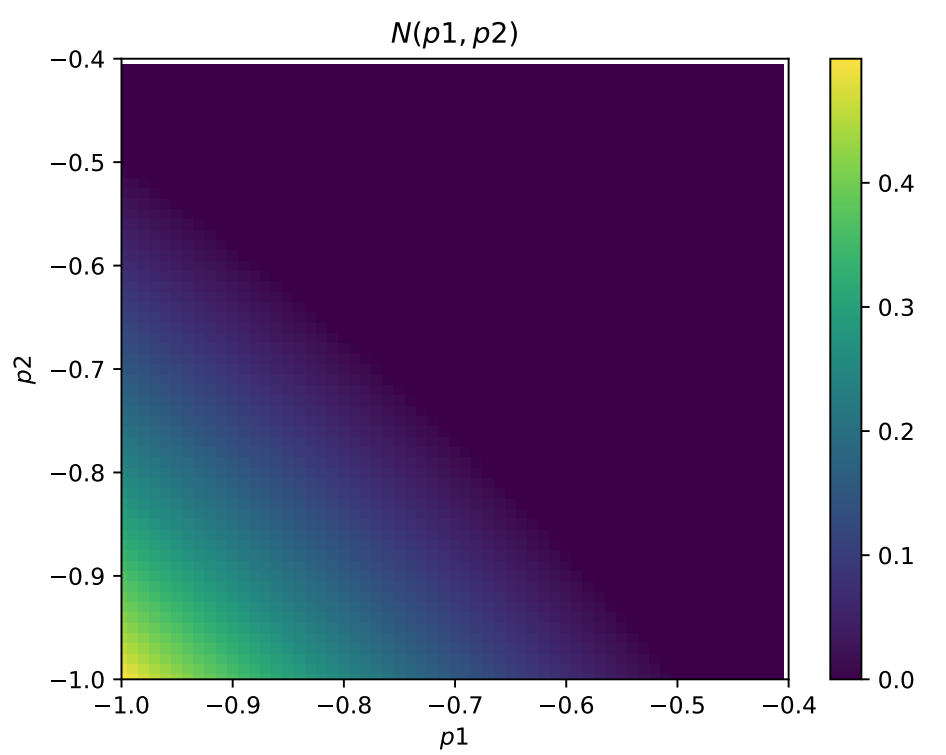
\includegraphics[width=0.7\linewidth]{img/2-werner-3d-simple.png}}
    \caption{
    Численный результат SDP задачи \ref{sdp-task-main} для 
    состояния $\rho_{wer}(p_1,2) \otimes \rho_{wer}(p_2,2)$ при разных значениях параметров $p_1$ и $p_2$. Точки, в которых $N(p_1, p_2) > 0$, соответствуют истинно сцепленным состояниям. По графику видно, что произведение сцепленных состояний не всегда является истинно сцепленным. Действительно, в противном случае график имел бы квадратную форму, а не треугольную.
    }
    \label{ris:sdp-2-warn-states}
\end{figure}

Проведем аналогичные вычисления с изотропным состоянием. \textbf{Изотропные состояния} - это семейство состояний, определенных на пространстве $\mathbb{C}^{d} \otimes \mathbb{C}^{d}$, которые инвариантны относительно унитарных преобразований следующего вида $U \otimes U^{*}$. Их можно параметризовать следующим образом
\begin{equation}\label{isotropic-state}
    \rho_{iso}(p, d) = p \ket{\phi^{+}_d}\bra{\phi^{+}_d} + \frac{1-p}{d^2}\mathbb{1},
\end{equation}
где $\ket{\phi^{+}_d}$ - $d$-мерное максимально сцепленное состояние $\ket{\phi^{+}_d} = \frac{1}{\sqrt{d}}\sum\limits_{i=0}^{d-1}\ket{ii}$.

При $d=2$ матрица плотности изотропного состояния будет иметь следующий вид
\begin{equation}\label{isotropic-state-2dmatrix}
    \rho_{iso}(p, 2) = \frac{1}{4}
    \begin{pmatrix}
        p+1 & 0 & 0 & 2p \\
        0 & p-1 & 0 & 0 \\
        0 & 0 & p-1 & 0 \\
        2p & 0 & 0 & p+1 \\
    \end{pmatrix}.
\end{equation}
Рассмотрим, как и в прошлый раз, цепочку из двух изотропных состояний $\rho_{iso}(p_1,2) \otimes \rho_{iso}(p_2,2)$ и построим аналогичный график. Результат представлен на рис. \ref{img:2-isotropic}а.

В статье \cite{Contreras_Tejada_2022} приводился аналитический анализ сцепленности изотропных состояний, в частности там было доказано, что цепочка из двух одинаковых изотропных состояний будет истинно сцепленной, если параметр $p$ будет удовлетворять следующему неравенству
\begin{equation}\label{isotropic-bisep-analitic-bound}
    p > \frac{(1 + \sqrt{2})d - 1}{d^2 + 2d - 1}.
\end{equation}
Для случая $d=2$ неравенство примет вид $p > 0.5469$. На рис. \ref{img:2-isotropic}a нарисована прямя $p_2 = p_1$, на которой изображена нижняя теоретическая граница. После нее состояние является истинно сцепленным. На срезе графика по прямой $p_2 = p_1$, представленным на рис. \ref{img:2-isotropic}b видно, что теоретическая граница и экспериментальная согласуются в пределах погрешности.

\begin{figure}
    \subfigure[]{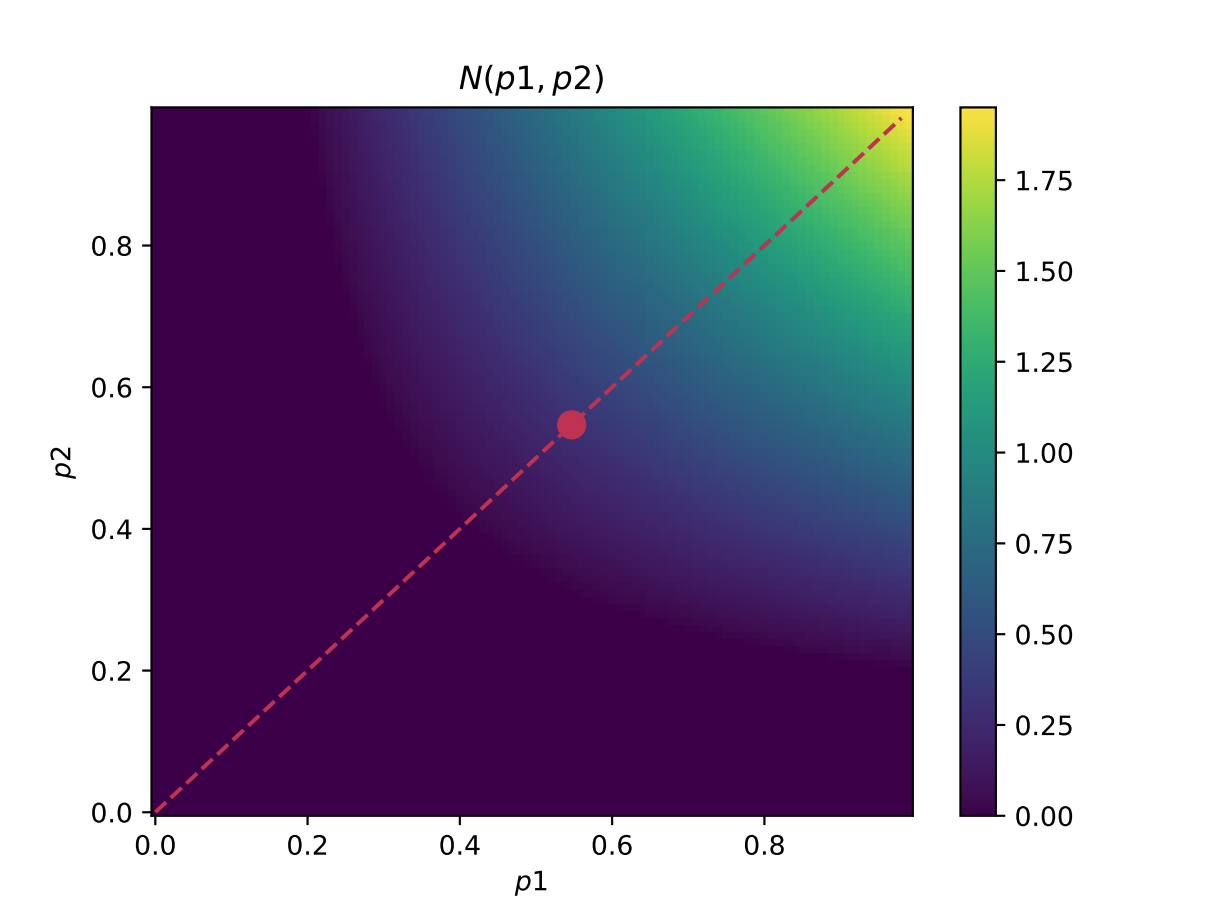
\includegraphics[width=0.55\textwidth]{img/2-isotropic-3d.png}}
    \subfigure[]{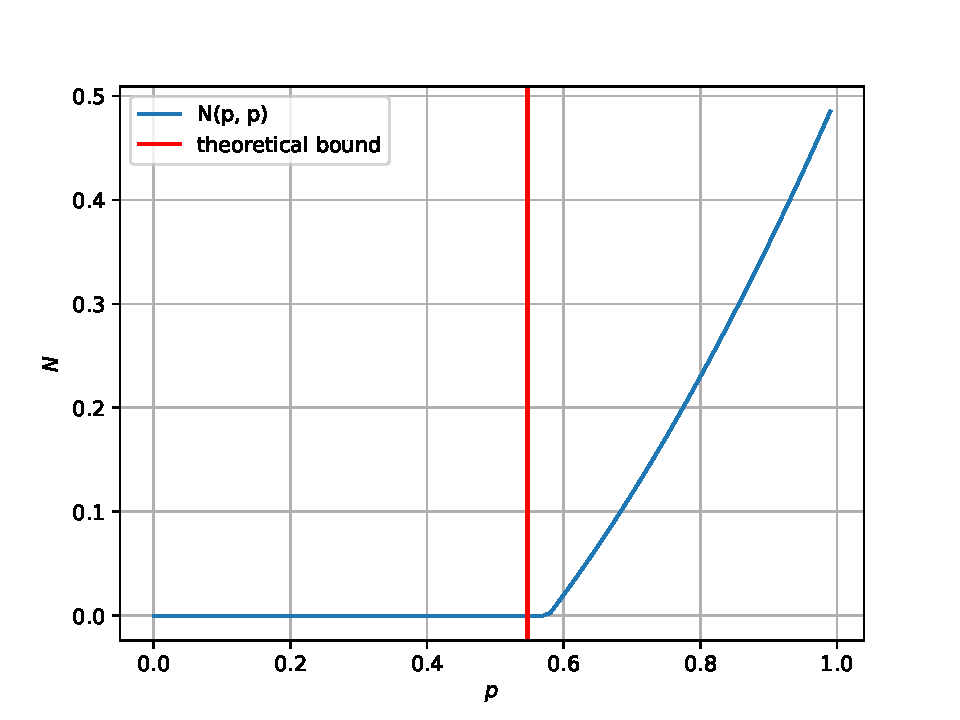
\includegraphics[width=0.55\textwidth]{img/2-isotropic-2d.pdf}}
    \subfigure[]{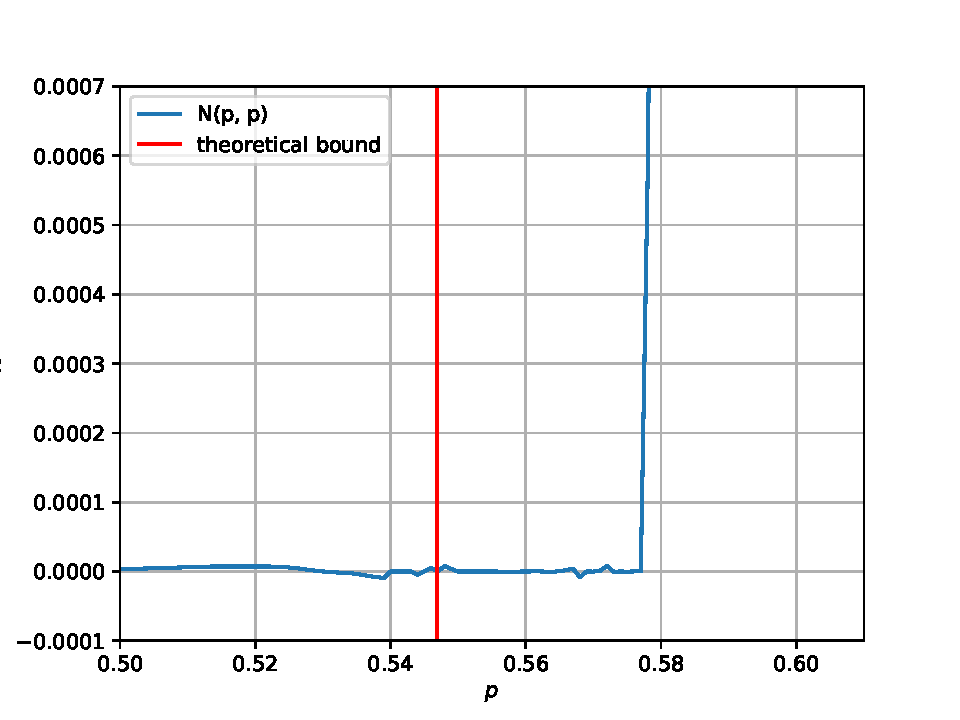
\includegraphics[width=0.55\textwidth]{img/2-isotropic-2d-detail.pdf}}
    \caption{
    \textbf{a} - численный результат SDP задачи \ref{sdp-task-main} для состояния $\rho_{iso}(p_1,2) \otimes \rho_{iso}(p_2,2)$ при разных значениях параметров $p_1$ и $p_2$. Точки, в которых $N(p_1, p_2) > 0$, соответствуют истинно сцепленным состояниям. Красная прямая $p_2 = p_1$ и точка на ней, показывает нижнюю теоретическую границу, после которой состояние является сцепленным.
    \textbf{b} - представлен срез графика a по прямой $p_2 = p_1$.
    \textbf{c} - представлен более детальный график b в точке излома.}
    \label{img:2-isotropic}
\end{figure}

Заметим, что аналитическую границу сцепленности \ref{isotropic-bisep-analitic-bound} можно применить и к семейству состояний Вернера.
Действительно, матрицу плотности для $d=2$ состояния Вернера можно представить в следующем виде
\begin{equation}
\begin{split}
    \rho_{wer}(p, 2) & = 
    \frac{1}{2(2 + p)}
    \begin{pmatrix}
        p+1 & 0 & 0 & 0 \\
        0 & 1 & p & 0 \\
        0 & p & 1 & 0 \\
        0 & 0 & 0 & p+1 \\
    \end{pmatrix}
     = \\
    &= \frac{\lambda}{4} \mathbb{1} + (1-\lambda)\ket{\psi^{-}_2} \bra{\psi^{-}_2}
     =
    \begin{pmatrix}
        \frac{\lambda}{4} & 0 & 0 & 0 \\
        0 & \frac{1-\lambda}{2} + \frac{\lambda}{4} & -\frac{1-\lambda}{2} & 0 \\
        0 & -\frac{1-\lambda}{2} & \frac{1-\lambda}{2} + \frac{\lambda}{4} & 0 \\
        0 & 0 & 0 & \frac{\lambda}{4} \\
    \end{pmatrix}, \\
\end{split}
\end{equation}

где $\ket{\psi^{-}_2}$ максимально смешенное состояние, $\ket{\psi^{-}_2} = \frac{1}{\sqrt{2}} \left( \ket{01} - \ket{10} \right)$ и $\lambda = \frac{2(p+1)}{2 + p}$.
С помощью унитарного преобразования $U$, которое не повлияет на сцепленности, можно перевести $\ket{\psi^{-}_2}$ в $\ket{\psi^{+}_2}$.
Тогда состояние Вернера, выраженное через максимально смешенное состояние, с точностью до коэффициентов, совпадет с 
 определением изотропного состояния \ref{isotropic-state}.
 Тогда теоретическую оценку границу сцепленности для изотропных состояний \ref{isotropic-bisep-analitic-bound} 
 можно примести и для состояния Вернера в случае, когда $d=2$
 \begin{equation}\label{werner-sep-2d-analytic-bound}
 \begin{split}
     & p < -\frac{2\beta(2)}{1 + \beta(2)} \approx -0.70709, \\
     & \beta(d) = \frac{(1 + \sqrt{2})d - 1}{d^2 + 2d - 1}.
 \end{split}
 \end{equation}

Сравнение полученного результата решения  SDP задачи с теоретической границей представлено на рис. \ref{img:2-werner-compare}.
\begin{figure}
    \subfigure[]{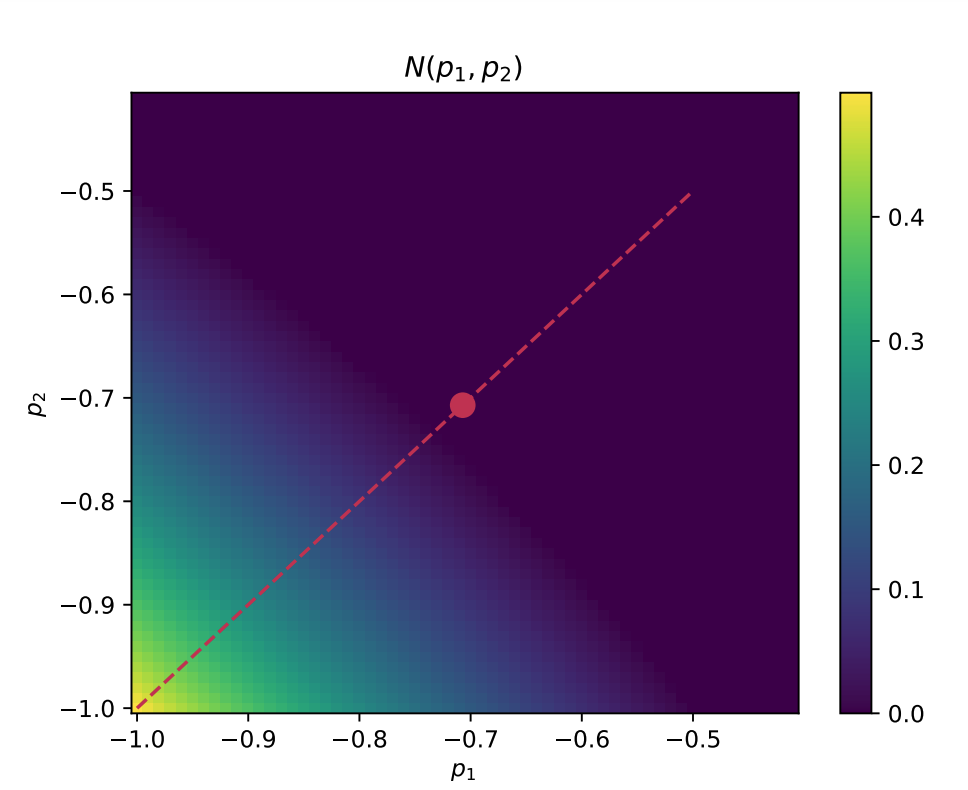
\includegraphics[width=0.55\textwidth]{img/2-werner-3d.png}}
    \subfigure[]{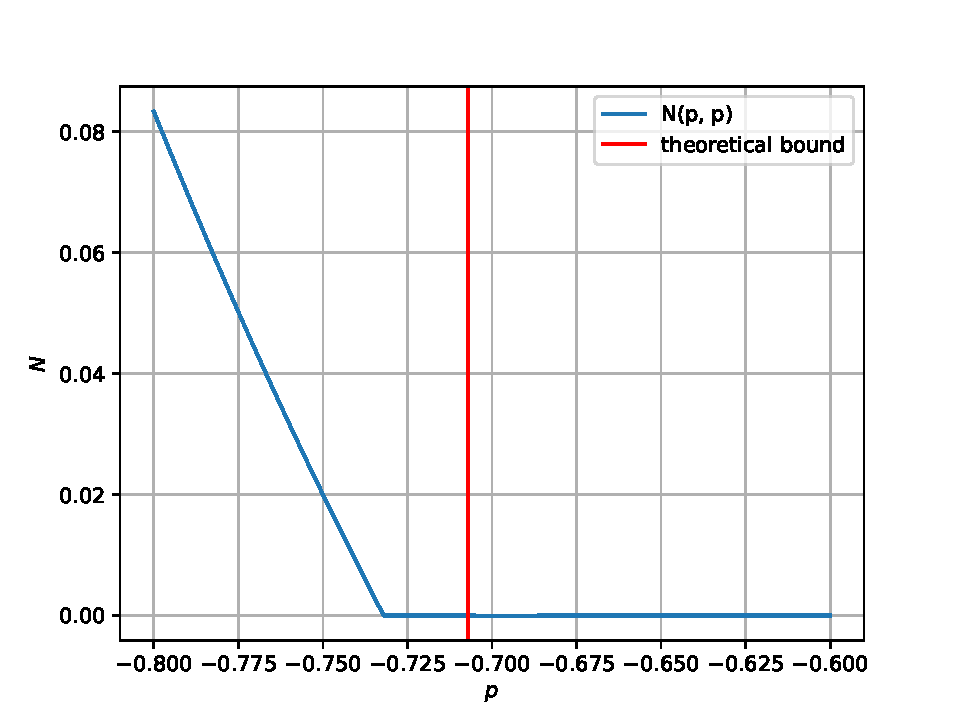
\includegraphics[width=0.55\textwidth]{img/2-werner-2d.pdf}}
    \subfigure[]{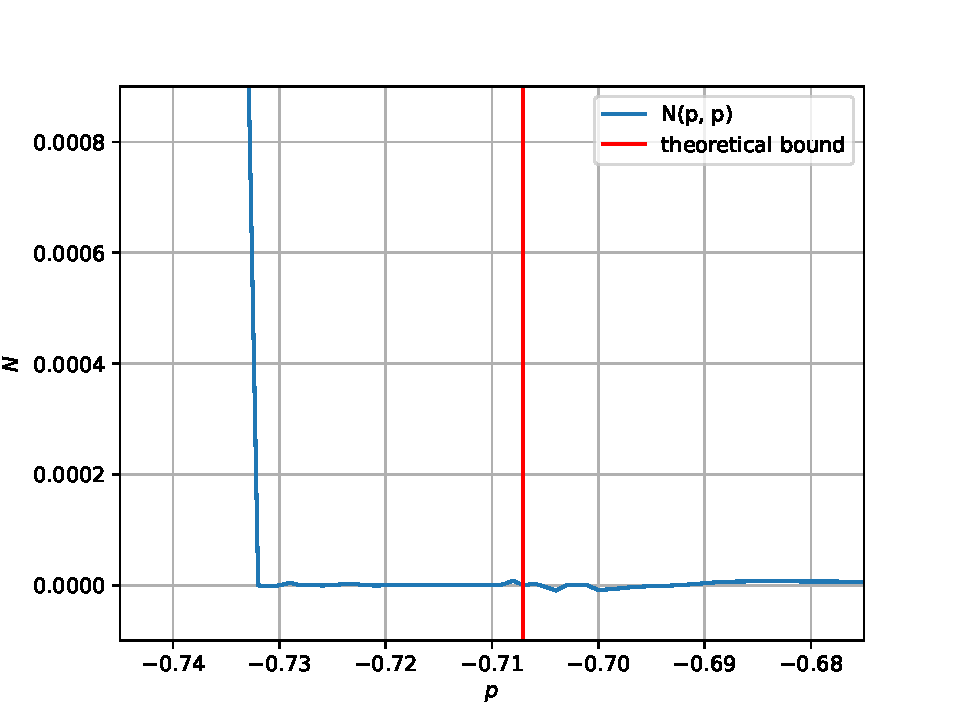
\includegraphics[width=0.55\textwidth]{img/2-werner-2d-detail.pdf}}
    \caption{
    \textbf{a} - численный результат SDP задачи \ref{sdp-task-main} для состояния $\rho_{wer}(p_1,2) \otimes \rho_{wer}(p_2,2)$ при разных значениях параметров $p_1$ и $p_2$. Точки, в которых $N(p_1, p_2) > 0$, соответствуют истинно сцепленным состояниям. Красная прямая $p_2 = p_1$ и точка на ней, показывает нижнюю теоретическую границу, после которой состояние является сцепленным.
    \textbf{b} - представлен срез графика \textbf{a} по прямой $p_2 = p_1$.
    \textbf{c} - представлен более детальный график \textbf{b} в точке излома.}
    \label{img:2-werner-compare}
\end{figure}

\chapter{Приложение}
\section{Частичное транспонирование.}
\label{appendix:partial_transpose}
Частичное транспонирование означает транспонирование по отношению к одной из подсистем. Рассмотрим пример, пусть матрица $\rho$ задает матрицу плотности для двух подсистем $H_A \otimes H_B$, тогда ее можно представить в виде $\rho = \sum\limits_{ijkl} p_{kl}^{ij} \ket{i}\bra{j} \otimes \ket{k} \bra{l}$. Тогда частичное транспонирование матрицы плотности $\rho$ относительно второй подсистемы $B$ можно будет записать с помощью оператора частичного транспонирования $\rho^{T_B} = (I \otimes T_B) \rho = \sum\limits_{ijkl} \ket{i}\bra{j} \otimes (\ket{k} \bra{l})^{T} =  \sum\limits_{ijkl} \ket{i}\bra{j} \otimes \ket{l} \bra{k}$. Операция частичного транспонирования выглядит нагляднее, если ее рассматривать через блочное представление. Пусть $\textbf{dim}(H_A) = n$, а $\textbf{dim}(H_B) = m$, тогда матрицу плотности можно записать в следующем виде
\begin{equation}
    \rho =
    \begin{pmatrix}
        A_{11} & A_{12} & ... & A_{1n} \\
        A_{21} & A_{22} & ... & A_{2n} \\
        \vdots &        & \ddots &     \\
        A_{n1} & A_{n2} & ... & A_{nn}
    \end{pmatrix},
\end{equation}
где $A_{ij}$ матрицы размером $m \times m$. Тогда $\rho^{T_B}$ будет выглядеть следующим образом
\begin{equation}
    \rho^{T_B} =
    \begin{pmatrix}
        A_{11}^T & A_{12}^T & ... & A_{1n}^T \\
        A_{21}^T & A_{22}^T & ... & A_{2n}^T \\
        \vdots &        & \ddots &     \\
        A_{n1}^T & A_{n2}^T & ... & A_{nn}^T
    \end{pmatrix}.
\end{equation}

Теперь рассмотрим конкретный пример двух-кубитное семейство состояний Вернера
\begin{equation}\label{2-qubit-warner-state}
\rho = \frac{1}{2(2 + p)} \left(
I_2 \otimes I_2 + p \sum\limits_{i,j = 0}^{1}\ket{i, j} \bra{j, i}
\right).
\end{equation}

В этом случае матрица плотности $\rho$ и её частичное транспонирование $\rho^{T_B}$ будут иметь следующий вид
\begin{equation}
    \rho = \frac{1}{4} 
    \begin{pmatrix}
        1-p & 0 &  0  & 0 \\
        0 & p+1 & -2p & 0 \\
        0 & -2p & p+1 & 0 \\
        0 & 0 & 0 & 1-p
    \end{pmatrix}
\end{equation}
\begin{equation}
    \rho^{T_B} = \frac{1}{4} 
    \begin{pmatrix}
        1-p & 0 &  0  & -2p \\
        0 & p+1 &  0 & 0 \\
        0 & 0 & p+1 & 0 \\
        -2p & 0 & 0 & 1-p
    \end{pmatrix}
\end{equation}


\printbibliography %Prints bibliography
\end{document}